\selectlanguage{ngerman}
\section{Grundlagen}\label{ch:Grundlagen}
% - Grundsätzlich nötig: Bildsensor (welche technischen Daten nötig), Controller(welche technischen Daten nötig), Speicherung relevanter Daten, Verbindung zwischen Controller und Ausgabegerät (Warum Flutter und Go)
% - Begründete Entscheidung der jeweiligen Hardware und Software (Nennen von Alternativen)
% - Anforderungen an die Objekterkennung (Genauigkeit, Performance)
In diesem Kapitel wird beschrieben, welche Hardware- und Software-Komponenten für die Umsetzung des Projektes nötig sind.
Außerdem wird darauf eingegangen, welche Anforderungen diese erfüllen müssen.

Zunächst wird ein Rechner benötigt, welcher genug Rechenleistung aufweist, um die Objekt\-erkennung der Autos umsetzen zu können.
Es wäre eine Lösung denkbar, bei welcher die Videoaufzeichnungen in eine Cloud gestreamt werden und dort weiterverarbeitet werden.
Da die Rechenleistung von Mini-Computern für solche Szenarien jedoch mittlerweile für eine Objekterkennung stark genug ist und eine direkte Verarbeitung des Videomaterials die Menge der zu übertragenden Datenmengen stark einschränkt, wird ein solches System bevorzugt.
Dieses benötigt eine Möglichkeit einen Kamera-Sensor anbringen zu können und eine Kommunikationsmöglichkeit über Ethernet oder WLAN.
Die Wahl fällt auf einen Raspberry~Pi~3~B+, da dieser bereits vorrätig ist und somit kein zusätzlicher finanzieller Aufwand entsteht.
Die Rechenleistung sollte mit einem 64 Bit Quad Core 1,4~GHz-Prozessor und 1~GB Arbeitsspeicher für das Projekt ausreichend sein \cite{pi3}.
Um Autos zu erkennen, wird weder eine hohe Auflösung, noch eine hohe Bildwiederholfrequenz benötigt.
Es gibt viele Alternativen, welche für die Umsetzung des Projektes denkbar wären.
Falls die Leistung des gewählten Mini-Computers nicht ausreicht, sollten Alternativen, wie Vertreter der NVIDIA Jetson- oder der ASUS Tinker Board-Reihe für das Projekt in Betracht gezogen werden \cite{jetson} \cite{tinkerBoard}.

Als Kamera-Sensor wird die, in Abbildung~\ref{fig:PiCAM} dargestellte, Raspberry Pi Camera in der Version 2.1 verwendet.
Diese wurde speziell für den Raspberry Pi entwickelt und liefert mit einem 8 Megapixel-Sensor eine ausreichende Bildqualität.
Videos können mit bis zu 1080p aufgezeichnet werden \cite{piCAM}.
Der Sensor kann direkt mit dem Mini-Computer, über den dafür vorgesehenen seriellen Schnittstellenanschluss, verbunden werden.
Aufgrund der einfachen Kommunikation zwischen Kamera und Raspberry Pi, sowie einer mehr als ausreichenden Bildqualität wurden als Alternativen lediglich andere Versionen der Pi Camera betrachtet.
Wegen der Verfügbarkeit und den nicht benötigten Vorteilen der anderen Modelle, wie weitere Blickfelder oder bessere Auflösungen, wurde in dieser Arbeit Version 2.1 der Raspberry Pi Camera verwendet.

\begin{figure}[h]
	\myImagePos{}
	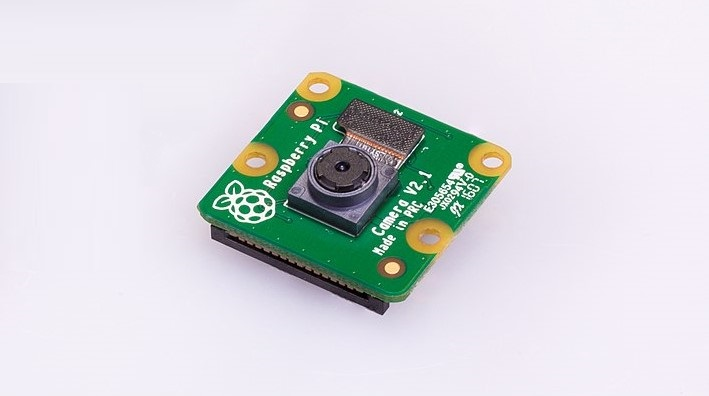
\includegraphics[width=0.4\myImageWidth]{Bilder/piCam.jpg}
	\caption[Raspberry Pi Camera V2.1]{Raspbarry Pi Camera V2.1 (Quelle: \cite{PiCamPIC})}
	\label{fig:PiCAM}
\end{figure}

Die Anzeige der Belegung des Parkhauses soll für Studenten und Mitarbeiter der Hochschule Coburg über ein beliebiges Endgerät aus erreichbar sein.
Aus diesem Grund ist es sinnvoll eine Multi-Plattform Applikation zu erstellen.
Diese sollte auf den gängigsten Betriebssystemen, wie Android, iOS, Windows oder im Web erreichbar sein.
Diese Anwendungen werden häufig durch Frameworks, wie Flutter, Xamarin (mittlerweile .NET MAUI) oder React Native, realisiert.
Die Wahl des verwendeten Frameworks fällt auf Flutter, da dies das aktuell modernste und verbreitetste Framework zur Erstellung nativer Multi-Plattform Anwendungen ist und außerdem bereits Erfahrungen mit dessen Programmierung gemacht wurden.
Die Realisierung mittels einer reinen Web-Anwendung wäre ebenfalls möglich gewesen.
Flutter bietet jedoch die Erstellung von sowohl Web-Anwendungen als auch Applikationen für verschiedene Betriebssysteme.

Als Bindeglied zwischen Raspberry Pi und Applikation für den Nutzer muss ein Server für das Handling der Daten implementiert werden.
Die Schnittstelle zum Server kann über HTTP-Anfragen realisiert werden.
Dieses Konzept ist weit verbreitet und Go, was zur Implementierung des Servers eingesetzt wurde, bietet hierfür hocheffiziente Bibliotheken.
Für die Schnittstelle zur Applikation ist es sinnvoll, eine Methode zu verwenden, welche es dem Server erlaubt, Daten zu schicken, ohne eine Anfrage zu erhalten.
So kann sichergestellt werden, dass die Anzeige der Anwendung stets mit dem Auslastungs-Wert des Servers übereinstimmt und hierfür kein Polling notwendig ist.
Ein dafür häufig verwendetes Protokoll, das auch in dieser Arbeit verwendet wird, ist MQTT.\@
